\section{Lecture 6, Synaptic plasticity and learning}
\begin{longtable}{p{4cm}p{15cm}}
Plasticity	& In this context, plasticity means the ability of synapses to change their properties, such that the synapse is strengthened or weakened.\\
Example		& \begin{tabular}[t]{l}
       		  	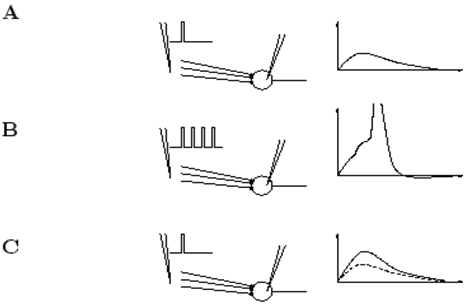
\includegraphics[width=10cm]{neuroinf_plasticity.png}\\
			Left side: Presynaptic spikes. Right side: Postsynaptic potentials\\
			A. Postsynaptic response before modification of synapse
			B. Strong presynaptic stimulation triggers postsynaptic firing
			C. Postsynaptic response after plasticity has occured.
       		  \end{tabular}\\
Hebb's Postulate	& When an axon of cell A is near enough to excite cell B or repeatedly or persistently takes part in firing it, some growth process or metabolic change takes place in one or both cells sucht that A's efficiency, as one of the cells firing B, is increased.\\
Strength of synapse	& The strength of a synapse can be defined by a variety of parameters:\\
			&   \begin{itemize}
			    	\item Neurotransmitter and receptor type (fixed)
				\item Position of synapse
				\item Availability of vesicles
				\item Neuromodulators
				\item Postsynaptic cellular processes
			    \end{itemize}\\
Weight of synapse	& After Hebbian learning, a synpase is strengthened, if presynaptic and postsynaptic cell fire simultaneously. In a neural network, the connection (the synapse) between two artificial neurons has a weight which models the strength of a synapse. For hebbian learning, this weight is defined as $w_{ij} = x_ix_j$ where $x_i, x_j$ are boolean and determine whether or not cell $i$ and $j$ fire for a specific training example.\\
Limitations of Hebbian Learning	& \begin{itemize}
                               	  	\item Only potentiation modeled (no depression)
					\item $\Rightarrow$ Leads to instability (positive feedback loops)
					\item Only variables locally available at the synapse are taken into account
                               	  \end{itemize}\\
Pavlovian Conditioning	& Pavlovian conditioning can be explained by Hebb's postulate: A dog smells food and accumulates saliva, i.e. neuron ``smelling food'' and neuron ``salivation'' are active. By adding a bell to the food, also neuron ``hearing a bell'' is activated. Since neuron ``salivation'' is still active, its synapse with the bell-neuron is strengthened, so that the dog still accumulates saliva, even if the food is taken away.\\
NMDA-Receptor		& \begin{itemize}
				\item Ligand-gated and voltage-gated. The NMDAR is initially blocked by Mg$^{2+}$ ions. It can be unblocked if the postsynaptic membrane is depolarized (by backpropagation, see STDP).
				\item If the channel is unblocked (i.e. on pre- and postsynaptic cell firing simultaneously), Ca$^{2+}$ can flow into the postsynaptic cell.
				\item The presynaptic cell emits Glutamate (agonist) and other Neurotransmitter (coagonists, e.g. glycine) that activate the NMDA channel.
				\item 10x more permeable to Ca$^{2+}$ compared to Na$+$ or K$^+$
				\item Strong / Weak NMDA receptor activation $\Rightarrow$ potentiation / depression of synapse
            		  \end{itemize}\\
AMPA receptor		& \begin{itemize}
				\item Most common receptor in the nervous system.
            		  	\item Unlike the NMDA receptor, the AMPA receptor is not initially blocked.
				\item Unlike NMDAR, AMPAR doesn't allow Ca$^{2+}$ influx.
				\item If the presynaptic cell fires, Glutamate activates the AMPA receptor and Na$^+$ flows into the postsynaptic cell, causing a potential difference which can help to remove the Mg$^{2+}$. But in general, this help alone can't remove the Mg$^{2+}$
				\item Given a Ca$^{2+}$ flux, more AMPA Receptors are built into the synapse, therefore strengthening the connection due to the above mentioned helper role of AMPA receptors.
            		  \end{itemize}\\
Short-term plasticity	& The strengthening or weakening of a synapse lasts for some short time (milliseconds to few minutes) only.\\
LTP			& Long Term Potentiation: A synapse is strengthened in a long time range. Experimentally, the presynaptic cell is made firing with a high frequency (called tetanus). It is then observed, that the EPSP's amplitude is very high for a long time.\\
LTD			& Long Term Depression: A synapse efficiency is weakened in a long time range\\
STDP			& Spike Time Dependent Potentiation: Whether the synapse is strengthened or weakened, is dependent on the time when a spike of the pre- or postsynaptic cell occurs ($Potentiation(t_{pre} - t_{post})$). Example: If the presynaptic cell fires a bit earlier thant the postsynaptic cell, the synapse is strengthened, otherwise weakened. For Hebb's rule, the potentiation is maximal, if $t_{pre} - t_{post} = 0$. STDP adds a temporal factor (or a direction of information) to Hebbian learning: The synapse is strengthened, if the input neuron spikes a little earlier than the output neuron.\\
			& 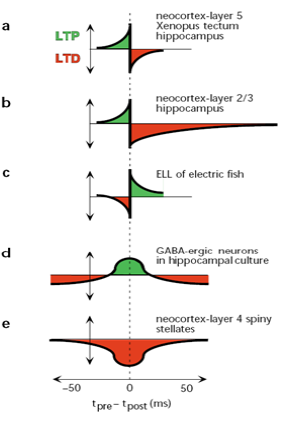
\includegraphics[width = 8cm]{neuroinf_stdp.png}\\
Dopamine		& Dopamine is a drug, which can raise the time range for LTP. Consequently, it is able to change prevent LTD and instead trigger LTP.\\
Factors that influence plasticity	& \begin{itemize}
                                 	  	\item Different plasticity in different brain areas
						\item Diversity in neurons and synapses
						\item Presynaptic spike frequency, postsynaptic membrane voltage, position of dendrites...
						\item Influence of neuromodulators, calcium, drugs, ...
						\item Short-term vs. Long-term effects
                                 	  \end{itemize}

\end{longtable}